%!TEX root = cscw2019-comic.tex

\section{Model Criticism}
\label{sec:Model Criticism}

In this section, we examine alternatives to the proposed model, a straightforward task in Bayesian analysis. We begin with a short section explaining our choice to use Bayesian analysis. Then in~\ref{sub:Posterior Checks, Convergence and Normality}, we examine how well the proposed models explains the observed data, including model convergence. Finally, in~\ref{sub:Alternative Models}, we examine alternative model formulations.

\subsection{Why Bayesian?}
\label{sub:Why Bayesian?}
In a recent paper,~\textcite{Kay2016}, make a persuasive argument that Bayesian methods are better suited to the HCI community, including making the case that Bayesian methods allow for replicating the results and improving the strength  of the conclusions by using previous outcomes as priors. We would add two reasons, in addition to those by~\textcite{Kay2016} to explain our decision to use Bayesian models. 
\begin{description}
    \item[Transparency:] With a Bayesian model, the researcher foregrounds all the aspects of the model; there are no modeling assumptions that need checking, not already foregrounded in the model description. Non-Bayesian statistics are powerful tools, and when used by an experienced statistician, they can dramatically reduce the process of inference. However, for researchers who wish to investigate their findings without access to a statistician, they need to be careful of the assumptions of the different tests: Normality ($t$-test); heteroscedasticity (e.g. ANOVA) and ensuring that the data satisfy the assumptions. Omitting the right sequence of analysis can lead to inferences not supported by the data.
    \item[Small $n$ studies:] A Bayesian model is valid at \textit{every} value of $n$; we do not have to wait for $n\geq 30$ to satisfy assumptions of say Normality. For small $n$ values, the result is of course affected by the choice of the prior; but by using weakly informative priors, we can ensure that the prior doesn't dominate inference. Furthermore, when Bayesian models use maximum entropy likelihood functions (e.g. members of the exponential family, that include the Normal distribution and the gamma distribution), we make the \textit{most conservative} inference given the data. See~\textcite[][Chapter 9]{McElreath2015} for an excellent description of the use of maximum entropy models in Bayesian analysis.
\end{description}


\subsection{Posterior Checks, Convergence and Normality}
\label{sub:Posterior Checks, Convergence and Normality}

In this section, we examine the model fits by examining how well the model makes predicts the observed data, model convergence and our assumptions about Normality.

\begin{figure*}[htb]
	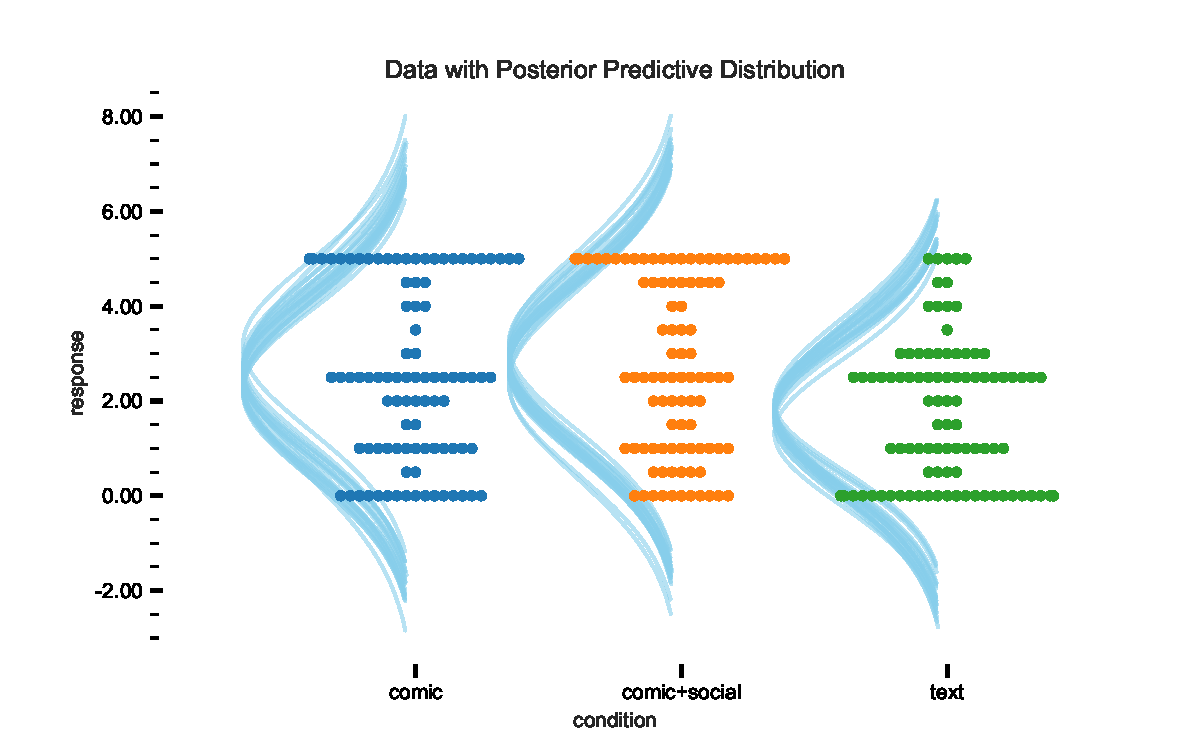
\includegraphics[width=1\textwidth]{./hari-code/posterior_predictions.pdf}
    \caption{Posterior prediction check: traces from the posterior distributions for each condition are super-imposed onto the observational data. The $x$-axis shows the three conditions, while the $y$-axis shows the contribution (each dot corresponds to a response by a single subject). The $t$-distribution captures the heavy tails, and we also see that the scale of the $t$-distribution in the case of the text condition is smaller than the other two cases. }
    \label{fig:posteriorprediction}
\end{figure*}

One of the advantages of a Bayesian model is that one can use the model to make predictions. Since the probabilistic model is generative, we can simply draw observations from the model. When we superimpose the posterior distribution traces onto the observational data in~\Cref{fig:posteriorprediction} we can observe three things. First, notice that the mean contribution for the `text' condition is less than the `comic' or the `comic+social norm' conditions, which seems reasonable given the increased number of \$0.0 contributions for the `text' condition in comparison to the other two cases. Second, the use of the heavy-tailed $t$-distribution captures well the tails of the distribution at \$0 and at \$5.0. Third, the scale of the distribution for the text condition is smaller than the scales for the two comic conditions, justifying our use of different scale parameters $\sigma_j$ for the three experimental conditions.

The model shows good convergence, as evidenced by the traceplot in~\Cref{fig:traceplot}.The Gelman-Rubin statistic $\hat{R}$ was around 1, indicating that the different sampling chains converged. Furthermore, the effective sample size of all parameters was greater than 10,000.

We used the $t$-distribution to model likelihood thinking that data may be heavy-tailed implying that a heavy-tailed distribution may be a better likelihood function than a  Normal distribution. Let us examine the posterior distribution for $\nu$, the degrees of freedom of the $t$-distribution. As a reminder, the $t$-distribution is equivalent to the Normal distribution when $\nu=\infty$. We can see that while the 95\% HPD lies between [17.37, 147.19], less than 7\% of the posterior lies below $\nu=30$, the traditional rule-of-thumb in non-Bayesian statistics for use of the Normal distribution.


\begin{figure}[htb]
    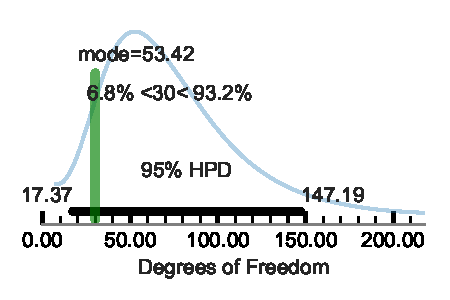
\includegraphics[width=0.5\textwidth]{./hari-code/robust_normality.pdf}
    \caption{The posterior distribution for $\nu$, the normality parameter of the $t$-distribution. When $\nu=\infty$ the $t$-distribution is identical to the Normal distribution. The posterior distribution shows a vertical green bar for $\nu=30$, the traditional cut-off condition for using a Normal distribution. The mode $\nu=53.42$, and the posterior probability distribution implies that only about 7\% of the posterior lies to the left of the green line (i.e. $P(\nu \leq 30) \approx 0.07$), implying that the assuming that the likelihood function to be Normally distributed will give similar inference.}
    \label{fig:normality}
\end{figure}

having discussed prediction checks, convergence and normality, next, we discuss alternatives to the model.

\subsection{Alternative Models}
\label{sub:Alternative Models}

As a first instance, consider a model similar model, except that the scale parameter of the likelihood function is drawn is \textit{not nested} like our current model, but is simply drawn from an uniform distribution $\sigma_j \sim U(L, H)$, where $L>0$ and where $H$ is a large constant.



